\chapter{Theory}
\section{Introduction}
\noindent  Modeling a WEC involves the interaction
between the incident waves, device motion, PTO mechanism,
and mooring (Figure \ref{fig:physics}). WEC-Sim uses a radiation and
diffraction method \cite{li2012synthesis,Babarit2012b} to predict
power performance and design optimization. The radiation and diffraction
method generally obtains the hydrodynamic forces from a frequency-domain
boundary element method (BEM) solver using linear coefficients to solve
the system dynamics in the time domain. \\

\begin{figure}[H]
\begin{centering}
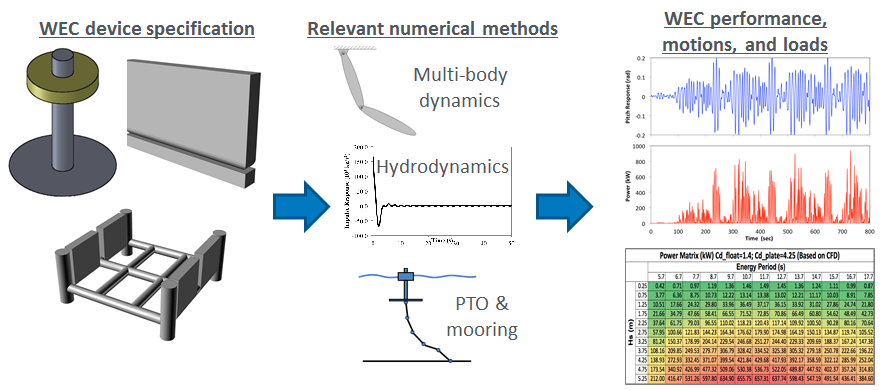
\includegraphics[scale=0.65]{theoryManual/Figures/Physics}
\end{centering}
\noindent \centering{}\protect\caption{Methodology for WEC-Sim\label{fig:physics}}
\end{figure}

\section{\noindent Boundary Element Method}
\noindent A common approach to determining the hydrodynamic forces is
to presume that they are the sum of incident, radiated, and diffracted wave components.
These forcing components are modeled using linear coefficients ideally obtained from a frequency-domain potential flow BEM solver (e.g., WAMIT \cite{Lee2006}, AWQA-FER \cite{_aqwa_}, and Nemoh
\cite{Nemoh2014}). The BEM solutions are obtained by solving the
Laplace equation for the velocity potential, which assumes the flow
is inviscid, incompressible, and irrotational. More details on the
theory for the frequency-domain BEM can be found in \cite{Lee2006}.

\section{\noindent Coordinate System in WEC-Sim}
Figure~\ref{fig:coordinate system} illustrates a 3-D floating point absorber subject to incoming waves in water. The figure also defines the coordinates and the 6 DOF in WEC-Sim. The WEC-Sim coordinate system  assumes that the  X axis is in the direction of wave propagation if the wave heading angle is equal to zero. The Z axis is in the vertical upwards direction, and the Y axis direction is defined by the right-hand rule. In the vectors and matrices used in the code, surge (x), sway (y), and heave (z) correspond to the first, second and third position respectively. Roll (Rx), Pitch (Ry), and Yaw (Rz) correspond to the fourth, fifth, and sixth position respectively.

\begin{figure}[H]
\begin{centering}
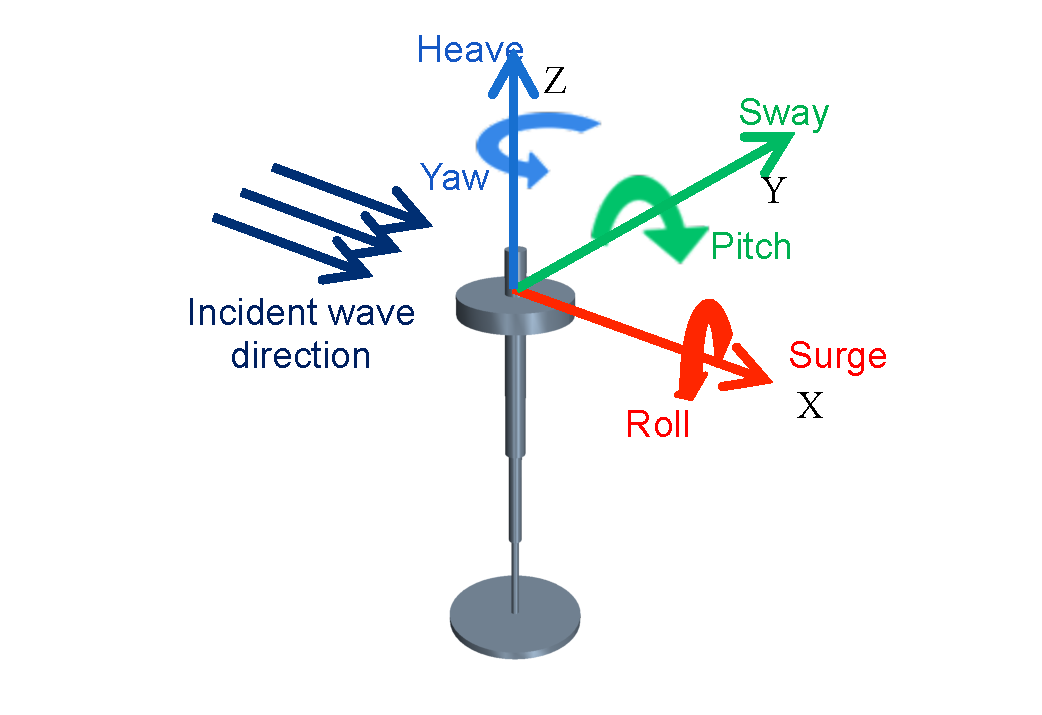
\includegraphics[scale=0.8]{theoryManual/Figures/coordinateSystem}
\end{centering}
\noindent \centering{}\protect\caption{Sketch defining the coordinate system\label{fig:coordinate system}}
\end{figure}

\section{\noindent Time-Domain Numerical Method}
\noindent The dynamic response of the system was calculated by solving
the equation of motion for WEC systems \cite{Babarit2012b,Nolte2014}. The equation of motion
for a floating body, about its center of gravity, can be given as:
\begin{equation}
m\ddot{X}=F_{ext}+F_{rad}+F_{PTO}+F_{v}+F_{B}+F_{m},
\end{equation}
where $\ddot{X}$ is the (translational and rotational) acceleration vector
of the device, $m$ is the mass matrix, $F_{ext}$ is the wave excitation
force vector, $F_{rad}$ is the force vector resulting from wave radiation,
$F_{PTO}$ is the PTO force vector, $F_{v}$ is the viscous damping
force vector, $F_{B}$ is the net buoyancy restoring force vector,
and $F_{m}$ is the force vector resulting from the mooring connection. 

\noindent Both $F_{ext}$ and $F_{rad}$ are calculated from values provided by the frequency-domain
BEM solver. The radiation term includes an added-mass and wave damping
term associated with the acceleration and velocity of the floating
body, respectively. The wave excitation term includes a Froude\textendash Krylov
force component generated by the undisturbed incident waves and a
diffraction component that results from the presence of the floating body. WEC-Sim
can be used for regular and irregular wave simulations, but note that
$F_{ext}$ and $F_{rad}$ are calculated differently for sinusoidal
steady-state response scenarios and random sea simulations. The sinusoidal
steady-state response is often used for simple WEC designs with regular
incoming waves. However, for random sea simulations or any simulations
where fluid memory effects of the system are essential, the convolution
integral method is recommended to represent the fluid memory retardation
force on the floating body. 

\subsection{\noindent Sinusoidal Steady-State Response Scenario}
\noindent This approach assumes that the system response is in sinusoidal
steady-state form, and is only valid for regular wave simulations.
The radiation term can be calculated using the added mass and the
wave radiation damping term for a given wave frequency, which is obtained
from
\begin{equation}
F_{rad}=-A(\omega_{r})\ddot{X}-B(\omega_{r})\dot{X},
\end{equation}
where $A(\omega_{r})$ and $B(\omega_{r})$ are the added-mass and
wave radiation damping matrices, respectively. $\omega_{r}$ is the wave frequency (in rad/sec),
and $\dot{X}$ is the velocity vector of the floating body. 

\noindent The free surface profile is based on linear wave theory
for a given wave height, wave frequency, and water depth. The regular
wave excitation force is obtained from
\begin{equation}
F_{ext}=\Re\left[ R_{f}\frac{H}{2}F_{X}(\omega_{r})e^{i(\omega_{r}t)} \right],\label{eq:RegularWaveExt}
\end{equation}

where $\Re$ denotes the real part of the formula, $R_{f}$ is the
ramp function, $H$ is the wave height, and $F_{X}$ is the excitation
vector, including the magnitude and phase of the force. 

\subsection{\noindent Convolution Integral Formulation}
\noindent To include the fluid memory effect on the system, the convolution
integral calculation, which is based upon the Cummins equation \cite{Cummins1962}, is used The
radiation term can be calculated by
\begin{equation}
F_{rad}=-A_{\infty}\ddot{X}-\intop_{0}^{t}K(t-\tau)\dot{X}(\tau)d\tau,
\end{equation}
where $A_{\infty}$ is the added mass matrix at infinite frequency and $K$ is the impulse response
function.

\noindent For regular waves, Eq. \ref{eq:RegularWaveExt} is used
to calculate the wave excitation force. For irregular waves, the free
surface elevation is constructed from a linear superposition of a
number of regular wave components. It is often characterized using
a wave spectrum (Figure \ref{fig:An-example-of PM Spectrum}) that
describes the wave energy distribution over a range of wave frequencies,
characterized by a significant wave height and peak wave period. The
irregular excitation force can be calculated as the real part of an
integral term across all wave frequencies as follows
\begin{equation}
F_{ext}=\Re\left[ R_{f} F_{X}(\omega_{r})e^{i(\omega_{r}t+\phi)} \intop_{0}^{\infty}\sqrt{2S(\omega_{r})d\omega_{r}} \right],
\end{equation}
where $S$ is the wave spectrum and $\phi$ is a random phase angle. 

\noindent 
\begin{figure}[h]
\noindent \begin{centering}
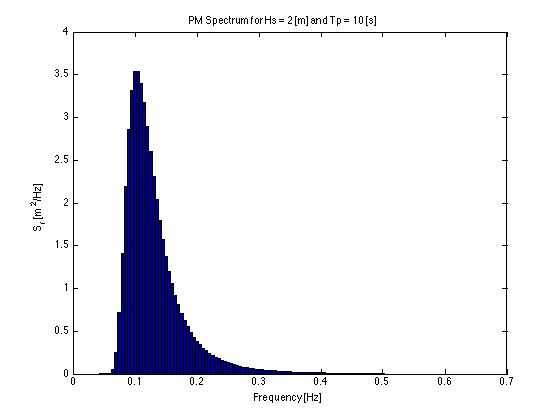
\includegraphics[scale=0.42]{theoryManual/Figures/Spectrum}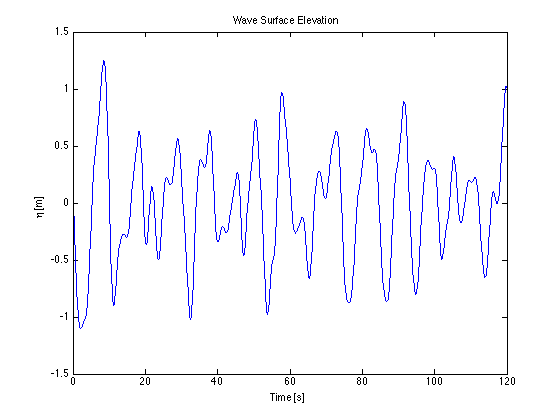
\includegraphics[scale=0.42]{theoryManual/Figures/WaveElevation}
\par\end{centering}
\noindent \centering{}\protect\caption{An example of wave spectrum and irregular wave elevation generated by WEC-Sim (Pierson\textendash Moskowitz spectrum)\label{fig:An-example-of PM Spectrum}}
\end{figure}

\subsection{Wave Spectrum}
The ability to generate regular waves provides an opportunity to observe the response of a model
under specific conditions. Sea states with constant wave heights and periods are rarely
found outside wave tank test. Normal sea conditions are more accurately represented
by random-wave time series that model the superposition of various wave forms with different 
amplitudes and periods. This superposition of waves is characterized by a sea spectrum.
Through statistical analysis, spectra are characterized by specific parameters such as significant
wave height, peak period, wind speed, fetch length, and others. The common
types of spectra that are used by the offshore industry are discussed in the following
sections.  The general form of the sea spectrums available in WEC-Sim is given by:
\begin{equation}
S\left( f \right) = A f^{-5}\exp\left[-B f^{-4} \right]~~,
\end{equation}
where $f$ is the wave frequency (in Hertz) and $\exp$ stands for the exponential function.

\subsubsection{Pierson--Moskowitz}
One of the simplest spectra was proposed by \cite{PM}. It assumed that after the wind blew steadily for a long time over a large area, the waves would come into equilibrium with the wind. This is the concept of a fully developed sea, where a "long time" is roughly 10,000 wave periods, and a "large area" is roughly 5,000 wave-lengths on a side.  The spectrum is calculated from
\begin{eqnarray}
& S\left( f \right) = \frac{\alpha_{PM}g^{2}}{\left( 2 \pi \right)^{4}}f^{-5}\exp\left[-\frac{5}{4} \left( \frac{f_{p}}{f}\right)^{4} \right]~~, &\\
& A = \frac{\alpha_{PM}g^{2}}{\left( 2 \pi \right)^{4}}~~, ~~ B = \frac{5}{4} {f_{p}}^{4}~~, &
\end{eqnarray}
where $\alpha_{PM}$ = 0.0081, $g$ is gravitational acceleration, and $f_{p}$ is the peak frequency of the spectrum.  However, this spectrum representation does not allow the user to define the significant wave height.  To facilitate the creation of a power matrix, in WEC-Sim the $\alpha_{PM}$ coefficient was calculated such that the desired significant wave height of the sea state was met.  The $\alpha_{PM}$ fit was calculated as follows:
\begin{eqnarray}
&\alpha_{PM} = \frac{H_{m0}^{2}}{16\int_{0}^{\infty} S^{*} \left( f \right) df}~~,&\\
& S^{*}\left( f \right) = \frac{ g^{2} }{ (2\pi)^{4}} f^{-5}\exp\left[-\frac{5}{4} \left( \frac{f_{p}}{f}\right)^{4} \right]~~. &
\end{eqnarray}
Note that related to the spectrum is a series of characteristic numbers called the spectral moments. These numbers, denoted $m_{k}~,~k=0, 1, 2,...$ are defined as
\begin{equation}
m_{k} = \int_{0}^{\infty} f^{k} S \left( f \right) df ~~.
\end{equation}
The spectral moment, $m_{0}$ is the variance of the free surface, which allows one to define
\begin{equation}
H_{m0} = 4 \sqrt{m_{0}}~~.
\end{equation}

\subsubsection{Bretschneider Spectrum}
This two-parameter spectrum is based on significant wave height and peak wave frequency.  For a
given significant wave height, the peak frequency can be varied to cover a range of conditions including developing and decaying seas. In general, the parameters depend on wind speed (most important),
wind direction, as well as fetch and locations of storm fronts. The spectrum is given as
\begin{eqnarray}
& S\left( f \right) = \frac{{H_{m0}}^2}{4}\left(1.057f_{p}\right)^{4}f^{-5}\exp\left[-\frac{5}{4} \left( \frac{f_{p}}{f}\right)^{4} \right]~~, &\\
& A =\frac{{H_{m0}}^2}{4}\left(1.057f_{p}\right)^{4} \approx \frac{5}{16} {H_{m0}}^2 {f_{p}}^{4}~~, &\\ 
& B = \left(1.057f_{p}\right)^{4} \approx \frac{5}{4} {f_{p}}^{4}~~, &
\end{eqnarray}
where $H_{m0}$ is the significant wave height which is generally defined as the mean wave height of the one third highest waves.

\subsubsection{JONSWAP (Joint North Sea Wave Project) Spectrum}
\textbf{\textit{Spectrum used in WEC-Sim}}\\
The spectrum was purposed by Hasselmann et al. \cite{HK},and  the original formulation was given as
\begin{eqnarray}
& S\left( f \right) = \frac{ \alpha_{j} g^{2} }{ (2\pi)^{4}} f^{-5}\exp\left[-\frac{5}{4} \left( \frac{f_{p}}{f}\right)^{4} \right]\gamma^\Gamma \nonumber & \\ 
&\Gamma = \exp \left[ -\left( \frac{\frac{f}{f_{p}}-1}{\sqrt{2} \sigma}\right)^{2} \right]~~, \sigma = \begin{cases} 0.07 & f \leq f_{p} \\ 
                                          0.09 & f > f_{p} \end{cases} ~~, &\\
& A =\frac{ \alpha_{j} g^{2} }{ (2\pi)^{4}}~~, ~~ B = \frac{5}{4} {f_{p}}^{4}~~, &
\end{eqnarray}
where $\alpha_{j}$ is a nondimensional variable that is a function of the wind speed and fetch length. 

Empirical fits were applied in an attempt to find a mean value that would capture the spectral shape of most measured sea states. To fit $\alpha_{j}$ to match the desired significant wave height the following calculation must be performed
\begin{eqnarray}
&\alpha_{j} = \frac{H_{m0}^{2}}{16\int_{0}^{\infty} S^{*} \left( f \right) df}~~,&\\
& S^{*}\left( f \right) = \frac{ g^{2} }{ (2\pi)^{4}} f^{-5}\exp\left[-\frac{5}{4} \left( \frac{f_{p}}{f}\right)^{4} \right]\gamma^\Gamma ~~. &
\end{eqnarray}

\textbf{\textit{Spectrum purposed at ITTC}}\\
Another form of JONSWAP spectrum was purposed at the 17th International Towing Tank Conference (ITTC). It was defined as
\begin{eqnarray}
& S\left( f \right) = \frac{155 }{ \left( 2\pi \right)^{4}} \frac{H_{m0}^{2}}{(0.834T_{p})^{4}} f^{-5}\exp\left[-\frac{5}{4} \left( \frac{f_{p}}{f}\right)^{4} \right]\gamma^\Gamma \nonumber & \\ 
& \approx \frac{310 }{ \left( 2\pi \right)^{4}} {H_{m0}}^{2} {f_{p}}^{4} f^{-5}\exp\left[-\frac{5}{4} \left( \frac{f_{p}}{f}\right)^{4} \right]\gamma^\Gamma~~, &\\
&\Gamma = \exp \left[ -\left( \frac{\frac{f}{f_{p}}-1}{\sqrt{2} \sigma}\right)^{2} \right]~~,~~ \sigma = \begin{cases} 0.07 & f \leq f_{p} \\ 
                                          0.09 & f > f_{p} \end{cases} ~~, \\
& A =\frac{310 }{ \left( 2\pi \right)^{4}} {H_{m0}}^{2} {f_{p}}^{4}~~, ~~ B = \frac{5}{4} {f_{p}}^{4}~~. &
\end{eqnarray}
Figure~\ref{fig:JONSWAP} shows the comparison of the JONSWAP spectrum obtained from the $\alpha_{j}$ fit and the ITTC description .  It is clear that the two methods have very good agreement.

\begin{figure}[h]
\begin{centering}
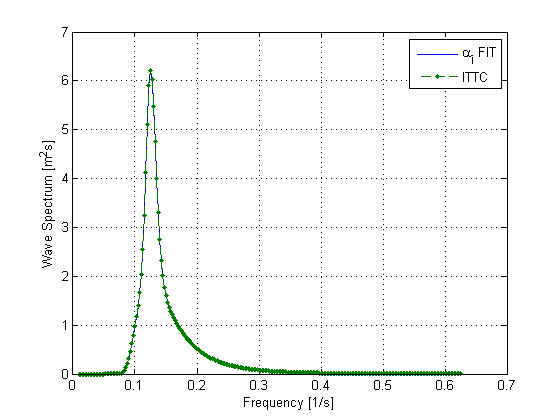
\includegraphics[scale=0.9]{theoryManual/Figures/Jonswap.png}
\end{centering}
\noindent \centering{}\protect\caption{Comparison of $\alpha_{j}$ fit to the ITTC description of the JONSWAP spectrum with $H_{m0}$ = 2 m and peak period ($T_{p}$) of 8 sec.\label{fig:JONSWAP}}
\end{figure}

\subsection{Ramp Function}
\noindent A ramp function ($R_{f}$), necessary to avoid strong transient
flows at the earlier time steps of the simulation, is used to calculate
the wave excitation force. The ramp function is given by
\begin{equation}
R_{f}=\begin{cases}
\frac{1}{2}(1+\cos(\pi+\frac{\pi t}{t_{r}}), & \frac{t}{t_{r}}<1\\
1, & \frac{t}{t_{r}}\geq1
\end{cases},
\end{equation}
where $t$ is the simulation time and $t_{r}$ is the ramp time.

\section{\noindent Power Take-off Forces}
\noindent The PTO mechanism is represented as a linear
spring-damper system, where the reaction force is given by: 
\begin{equation}
F_{PTO}=-K{}_{PTO}X_{rel}-C_{PTO}\dot{X}_{rel},
\end{equation}
where $K_{PTO}$ is the stiffness of the PTO, $C_{PTO}$ is the damping
of the PTO, and $X_{rel}$ and $\dot{X}_{rel}$ are the relative motion
and velocity between two bodies.  The power consumed by the PTO is given by:
\begin{equation}
P_{PTO} = -F_{PTO}\dot{X}_{rel}=\left(K_{PTO}X_{rel}\dot{X}_{rel}+C_{PTO}\dot{X}^{2}_{rel}\right).
\end{equation}
However, the relative motion and velocity between two bodies is out of phase by $\pi/2$, resulting in a time-averaged product of 0. This allows the absorbed power to be written as
\begin{equation}
P_{PTO} =C_{PTO}\dot{X}^{2}_{rel}.
\end{equation}

\section{\noindent Mooring Forces}
\noindent The mooring load is represented using a linear quasi-static
mooring stiffness, which can be calculated by
\begin{equation}
F_{m}=-K_{m}X,
\end{equation}
where $K_{m}$ is the stiffness matrix for the mooring system, and
$X$ is the response of the body.

\section{Viscous Drag}
\noindent Generally, the effect of viscosity on the WEC dynamics needs
to be considered as neglecting this effect may lead to an overestimation
of the power generation of the system, particularly when a linear
model is applied. A common way of modeling the viscous damping is
to add a (Morison-equation-type) quadratic damping term to the equation
of motion;
\begin{equation}
F_{V}=\frac{1}{2}C_{d}\rho A_{D}\dot{X}|\dot{X}|,
\end{equation}
where $C_{d}$ is the viscous drag coefficient, $\rho$ is the fluid density, and $A_{D}$ is the
characteristic area. The viscous drag coefficient for the device
must be carefully selected \cite{li2012synthesis,Babarit2012b}; however, it
is dependent on device geometry, scale, and relative
velocity between the body and the flow around it. The drag coefficient
becomes much larger when the Reynolds and the Keulegan\textendash Carpenter
number are smaller. Note that empirical data on the drag
coefficient can be found in various literature and standards. The available data may, 
however, be limited to existing simple geometries. For
practical point absorber geometry, the hydrodynamic forces may have
to be evaluated by conducting wave tank tests or prescribed motion
computational fluid dynamic simulations.
